\documentclass[russian,utf8,emptystyle]{eskdtext}

\newcommand{\No}{\textnumero} % костыль для фикса ошибки

\ESKDdepartment{Федеральное государственное бюджетное образовательное учреждение высшего профессионального образования}
\ESKDcompany{Московский государственный технический университет им. Н. Э. Баумана}
\ESKDclassCode{23 0102}
\ESKDtitle{Домашнее задание №3 по дисциплине}
\ESKDdocName{<<Теоретические основы реляционной алгебры>>}
\ESKDauthor{Гуща~А.~В.}
%\ESKDtitleApprovedBy{к.т.н. доцент}{Григорьев Ю.А.}
%\ESKDtitleAgreedBy{к.т.н. доцент}{Григорьев Ю.А.}
\ESKDtitleDesignedBy{Студент группы ИУ5-92}{Гуща~А.~В}

\usepackage{multirow}
\usepackage{tabularx}
\usepackage{tabularx,ragged2e}
\usepackage{pdfpages}
\usepackage{pdflscape}
\renewcommand\tabularxcolumn[1]{>{\Centering}p{#1}}
\newcommand\abs[1]{\left|#1\right|}

\usepackage{longtable,tabu}

\usepackage{geometry}
\geometry{footskip = 1cm}

\pagenumbering{arabic}
\pagestyle{plain}

\usepackage{setspace}
\usepackage{enumitem}

\usepackage{xcolor}
\usepackage{amssymb}
\usepackage{listings}
\lstset{
    breaklines=true,
    postbreak=\raisebox{0ex}[0ex][0ex]{\ensuremath{\color{red}\hookrightarrow\space}},
    extendedchars=\true,
    basicstyle=\small,
    inputencoding=utf8
}

\begin{document}
\maketitle
%\includepdf[pages={1}]{title.pdf}

\tableofcontents
\clearpage

\section{Постановка задачи}

Выдать имена поставщиков из Лондона, которые поставляют для изделия с номером <<J1>>, по крайней мере, одну красную деталь.

Задание:
\begin{enumerate}[label=\arabic*.]
\item Написать соответствующий оператор SELECT и построить логический план выполнения этого оператора
\item Определить оптимальный физический план выполнения оператора SELECT при следующих исходных данных:
\begin{enumerate}[label=\arabic*)]
\item Количество записей в таблице:
$$
T(S) = 10000
$$
$$
T(P) = 100000
$$
$$
T(SPJ) = 1000000
$$
\item Количество записей в одном блоке таблицы:
$$
L_S = 500
$$
$$
L_P = 500
$$
$$
L_{SPJ} = 1000
$$
$$
L_{JOIN} = 2000
$$
\item Индексы атрибутов и число записей таблицы в одном блоке индекса (L):
\begin{itemize}
\item таблица S: 
\begin{enumerate}[label=\arabic*)]
\item индекс по атрибуту <<$N_\text{пост}$>>, L = 200
\end{enumerate}
\item таблица P:
\begin{enumerate}[label=\arabic*)]
\item индекс по атрибуту <<$N_\text{дет}$>>, L = 200
\end{enumerate}
\item таблица SPJ:
\begin{enumerate}[label=\arabic*)]
\item индекс по атрибуту <<$N_\text{пост}$>>, L = 200
\item индекс по атрибуту <<$N_\text{дет}$>>, L = 200
\item индекс по атрибуту <<$N_\text{изд}$>>, L = 200
\end{enumerate}
\end{itemize}
\end{enumerate}

Примечения:
\begin{itemize}
\item записи таблиц могут читаться в отсортированном виде по своим индексированным атрибутам
\item записи во всех таблицах не сгруппированы (нет кластеризации)
\end{itemize}

\item Мощности атрибутов:
$$
I(S,\text{город}) = 50
$$
$$
I(S,N_\text{пост}) = 10000
$$
$$
I(P,\text{цвет}) = 20
$$
$$
I(P,N_\text{дет}) = 100000
$$
$$
I(SPJ,N_\text{пост}) = 5000
$$
$$
I(SPJ,N_\text{дет}) = 100000
$$
$$
I(SPJ,N_\text{изд}) = 10000
$$

\item Число блоков $B = 10$, значения:
$$
C_{comp} = C_{move} = C_{filter} = 0.01 \; \text{мс}
$$
$$
C_B = 10 \; \text{мс}
$$

\item Предполагается, что используются левосторонние деревья для поиска оптимального плана и применяются каналы. Примечание: рассматирвается метод NLJ (Nested Left Joins).
\end{enumerate}

\begin{figure}[h!]
\centering
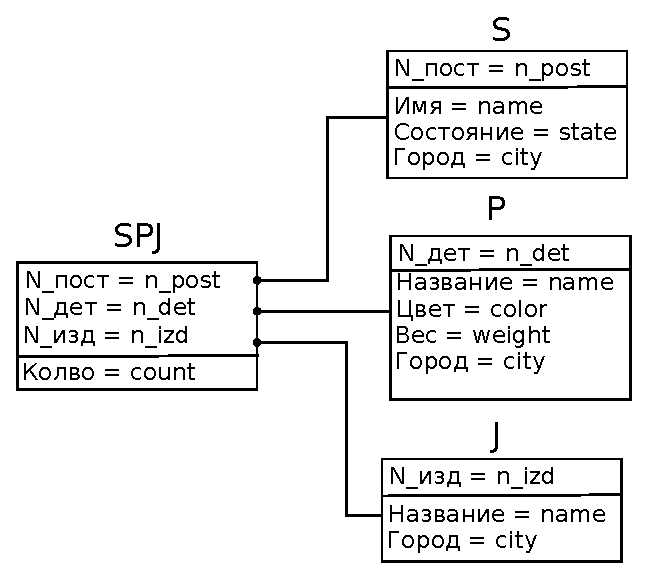
\includegraphics[width=0.8\textwidth]{sheme}
\caption{Схема базы данных c переименнованными атрибутами}
\label{fig:sheme}
\end{figure}

\section{Выполение}
\subsection{Оператор SELECT}
\begin{verbatim}
select S.name from SPJ, P, S
  where SPJ.n_det = P.n_det
    and SPJ.n_post = S.n_post
    and SPJ.n_izd = 'J1'
    and P.color = 'red'
    and SPJ.count >= 1
    and S.city = 'London'
\end{verbatim}

\subsection{Форма реляционной алгебры}
Используемые законы:
\begin{enumerate}[label=\arabic*.]
\item Закон каскада селекций:
$$
\sigma_{f_1 \wedge f_2}(R) = \sigma_{f_1}(\sigma_{f_2}(R))
$$
\item Закон перестановки селекции и декартового произведения:
$$
\sigma_{f_1}(R_1 \times R_2) = \sigma_{f_1}(R_1) \times R_2
$$
$$
attr(f_1) \in R_1 \wedge attr(f_1) \notin R_2
$$
\item Закон перестановки проекции и селекции:
$$
\Pi_{a_1 .. a_n}(\sigma_f(R)) = \Pi_{a_1 .. a_n}(\sigma_f(\Pi_{a_1..a_nb_1..b_k}(R))
$$
\item Закон перестановки проекции и декартнового произведения:
$$
b_1 .. b_n \in R_1
$$
$$
c_1 .. c_n \in R_2
$$
$$
\Pi_{b_1 .. b_nc_1 .. c_k}(R_1 \times R_2) = \Pi_{b1 .. b_n}(R_1) \times \Pi_{c_1 .. c_k}(R_2)
$$
\end{enumerate}

Преобразуем оператор SELECT в форму реляционной алгебры:
\begin{align*}
Q &= \Pi_{s.name}(\sigma_{spj.ndet = p.ndet \wedge spj.npost = s.npost \wedge spj.nizd='J1' \wedge p.color='red' \wedge} \\
  & \;_{ \wedge spj.count>=1 \wedge s.city='London' }(SPJ \times P \times S))
\end{align*}

Применяем закон каскада селекций:
\begin{align*}
Q &= \Pi_{s.name}(\sigma_{spj.ndet = p.ndet \wedge spj.npost = s.npost}( \\
  &  \sigma_{spj.nizd='J1' \wedge p.color='red' \wedge spj.count>=1 \wedge s.city='London'}(SPJ \times P \times S))
\end{align*}

Применяем закон перестановки селекции и декартового произведения:
\begin{align*}
Q &= \Pi_{s.name}(\sigma_{spj.ndet = p.ndet \wedge spj.npost = s.npost}( \\
  & (\sigma_{spj.nizd='J1' \wedge spj.count>=1}(SPJ) \times \sigma_{p.color='red'}(P) \times \sigma_{s.city='London'}(S)))
\end{align*}

Применяем закон перестановки проекции и селекции:
\begin{align*}
Q &= \Pi_{s.name}(\sigma_{spj.ndet = p.ndet \wedge spj.npost = s.npost}( \\
  & \Pi_{s.name, spj.ndet, p.ndet, spj.npost, s.npost}( \\
  & \sigma_{spj.nizd='J1' \wedge spj.count>=1}(SPJ) \times \sigma_{p.color='red'}(P) \times \sigma_{s.city='London'}(S))))
\end{align*}

Применяем закон перестановки проекции и декартового произведения:
\begin{align*}
Q &= \Pi_{s.name}(\sigma_{spj.ndet = p.ndet \wedge spj.npost = s.npost}( \\
  & \Pi_{spj.ndet,spj.npost}(\sigma_{spj.nizd='J1' \wedge spj.count>=1}(SPJ)) \times \\
  & \Pi_{p.ndet}(\sigma_{p.color='red'}(P)) \times \\ 
  & \Pi_{s.name,s.npost}(\sigma_{s.city='London'}(S)) ))
\end{align*}

Выделяем подзапросы:
\begin{align*}
Q   &= \Pi_{s.name}(\sigma_{spj.ndet = p.ndet \wedge spj.npost = s.npost}( Q_1 \times Q_2 \times  Q_3 )) \\
Q_1 &= \Pi_{spj.ndet,spj.npost}(\sigma_{spj.nizd='J1' \wedge spj.count>=1}(SPJ)) \\
Q_2 &= \Pi_{p.ndet}(\sigma_{p.color='red'}(P)) \\
Q_3 &= \Pi_{s.name,s.npost}(\sigma_{s.city='London'}(S))
\end{align*}

\clearpage
\subsection{Логический план}
\begin{figure}[h!]
\includegraphics[width=0.9\textwidth]{logic_plan}
\caption{Логический план запроса}
\label{fit:logic_plan}
\end{figure}

\clearpage
\subsection{Выбор порядка соединений}
\begin{figure}[h!]
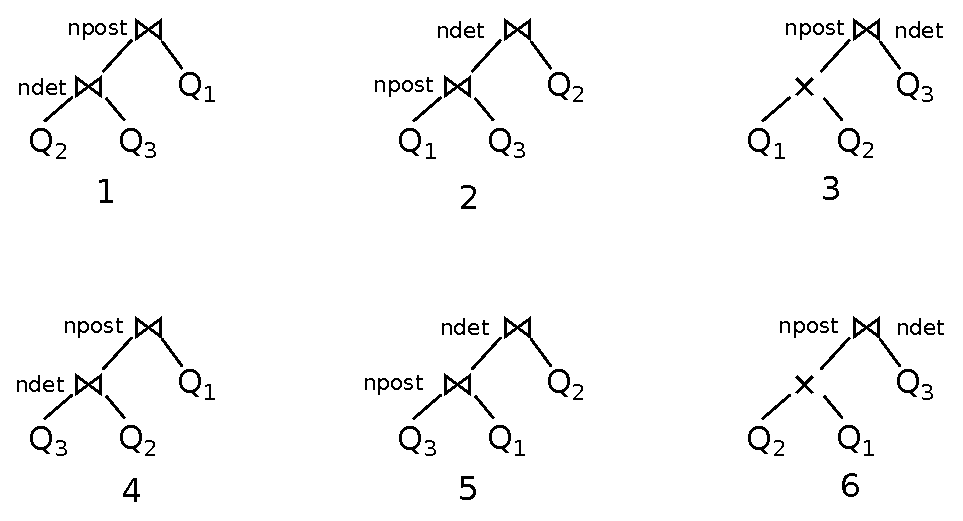
\includegraphics[width=0.9\textwidth]{join_variants}
\caption{Варианты соединения таблиц}
\label{fig:join_variants}
\end{figure}

Варианты 3 и 6 не рассматриваются в алгоритме, так как там используется декартовое произведение, что заведомо хуже других вариантов. Переномеруем варианты соединения, исключая 3 и 6.

\clearpage
\begin{figure}[h!]
\centering
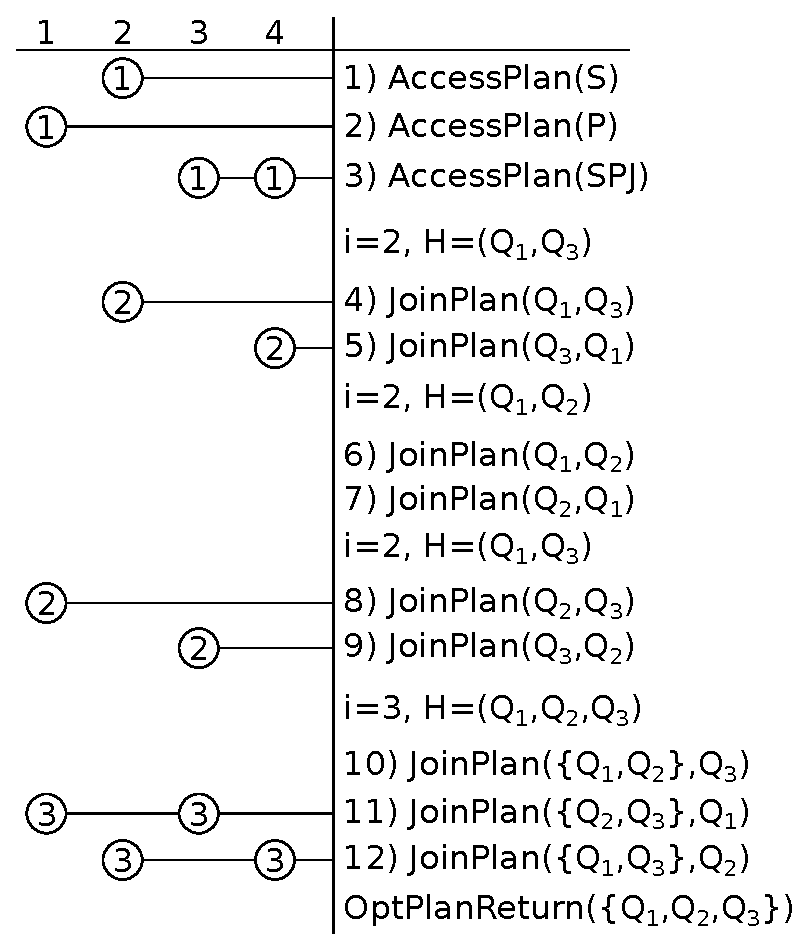
\includegraphics[width=0.9\textwidth]{join_plan_table}
\caption{Схема алгоритма на основе динамического программирования}
\label{fig:logic_plan_table}
\end{figure}

Варианты 1 и 2 не рассматриваются, так как в них потребуется полное сканирование таблиц из-за соединения по аттрибутам, для которых не построены индексы.

Итого из рисунка~\ref{fig:join_variants} рассматриваются варианты 4 и 5. Посчитаем условную стоимость (единицу измерения примем в миллисекундах) выполнения каждого из вариантов соединения таблиц.

\subsubsection{Вариант 4}

\paragraph{AccessPlan(SPJ)}:
\begin{enumerate}[label=\arabic*)]
\item Чтение всех SPJ, TableScan(SPJ):
\begin{align*}
C_1 &= C_{cpu1} + C_{io1} = T(SPJ)C_{filter} + \frac{T(SPJ)}{L_{SPJ}}C_B = \\
& = 20000 \; \text{мс}
\end{align*}
Где:
\begin{itemize}
\item $C_{cpu1}$ - оценка стоимости обработки на ЦПУ в миллисекундах
\item $C_{io1}$ - оценка стоимости операций ввода-вывода в миллисекундах
\item $T(SPJ)$ - количество строк в таблице SPJ
\item $L_{SPJ}$ - количество записей в одном блоке таблицы SPJ
\item $C_{filter}$ - стоимость фильтрации одной строки в миллисекундах
\item $C_B$ - стоимость чтения одной строки в миллисекундах
\end{itemize}
\item Чтение по индексу, IndexScan(SPJ, nizd):
\begin{align*}
C_2 &= C_{cpu2} + C_{io2} = \frac{T(SPJ)k}{I(SPJ,nizd)}C_{filter} + \\
& + \left(\left\lceil \frac{\frac{T(SPJ)}{L} k}{I(SPJ, nizd)} \right\rceil + \left\lceil \frac{T(SPJ) k}{I(SPJ, nizd)} \right\rceil \right) C_B = \\
& = 1011 \; \text{мс}
\end{align*}
Где:
\begin{itemize}
\item $L$ - число записей в одном блоке индекса
\item $L_{SPJ}$ - количество записей в одном блоке таблицы SPJ
\item $k$ - мощность атрибута в запросе
\item $I(SPJ, nizd)$ - мощность атрибута nizd в таблице SPJ
\end{itemize}
\end{enumerate}

Выбираем способ с минимальной оценкой:
$$
C = \min(C_1, C_2) = C_2 = 1011
$$
Оценка стоимости операций ввода-вывода:
$$
C_{io} = 1010
$$

Считаем количество строк в промежуточной таблице:
$$
T(Q_3) = T(SPJ)p_{nizd} = T(SPJ)\frac{k}{I(SPJ,nizd)} = 100
$$
Где $p_{nizd}$ - вероятность того, что строка в SPJ удовлетворит условию фильтрации.

Количество блоков в промежуточной таблице:
$$
B(Q_3) = \left\lceil \frac{T(Q_3)}{L_{SPJ}B} \right\rceil = 1
$$

Заполняем промежуточную структуру:
$$
str[1] = \{Q_3, \varnothing, \varnothing, 1011, 1010, \{100, 1, \{ndet, 100\}, nizd\}\}
$$

Данная структура имеет следующие поля:
\begin{itemize}
\item W - кортеж из таблиц или таблица, которая получается в результате операции (соединения)
\item X - левый аргумент операции
\item Y - правый аргумент операции
\item Z - оценка времени совокупная
\item ZIO - оценка времени ввода-вывода
\item V - подструктура:
\begin{itemize}
\item T - оценка количества строк в новой таблице
\item I - оценка количества блоков в новой таблице
\item подструктура, содержащая индекс, по которому будет проводится следующее соединение и мощность этого атрибута, которое считается как $\min(T(Q), I(R, atr))$, где R - исходная таблица, Q - промежуточная таблица
\item K - атрибут-индекс, по которому происходило объединение
\end{itemize}
\end{itemize}

\paragraph{JoinPlan($Q_3$,$Q_2$)}
\begin{enumerate}[label=\arabic*.]
\item Для $Q_3$:
$$
N = T(Q_3) = str[1].V.T = 100
$$
Для каждой полученной записи в $Q_3$ выполняется поиск в индексе по номеру детали в P.

\begin{align*}
C &= N \left( \frac{T(P)k}{I(P,ndet)}C_{filter} + \left(\left\lceil \frac{\frac{T(P)}{L_P}k}{I(P,ndet)} \right\rceil + \left\lceil \frac{T(P)k}{I(P,ndet)} \right\rceil \right) C_B \right) \\ 
&= 2000 \; \text{мс}
\end{align*}
$$
T(Q_2) = T(P) \frac{str[1].V.T}{I(P,ndet)} p_{color='red'} = 5
$$
$$
B(Q_2) = \left\lceil \frac{T(Q_2)}{L_P B} \right\rceil = 1
$$
$$
str[2] = \{Q_2, \varnothing, \varnothing, 2000, 2000, \{ 5, 1, \{ ndet, 5\}, ndet\}\}
$$

\item Для $Q_3 \bowtie Q_2$:

$$
m_1 = 1, \; m_2 = 2
$$

$$
C = str[1].Z + str[2] = 1011 + 2000 = 3011
$$
$$
C_{io} = str[1].ZIO + str[2] = 1010 + 2000 = 3010
$$
$$
T(Q_3 \bowtie Q_2) = T(Q_2) = str[2].V.T = 5
$$
$$
B(Q_3 \bowtie Q_2) = \left\lceil \frac{T(Q_3 \bowtie Q_2)}{L_{JOIN}} \right\rceil = 1
$$

$$
str[3] = \{ (Q_3, Q_2), Q_3, Q_2, 3011, 3010, \{ 5, 1, \{ \{ nizd, 5 \}\}, ndet\} \}
$$
\end{enumerate}

\paragraph{JoinPlan($\{Q_3, Q_2\}$, $Q_1$)}

\begin{enumerate}[label=\arabic*.]
\item $\{ Q_3, Q_2 \}$
$$
V = T(Q_3 \bowtie Q_2) = str[3].V.T = 5
$$
$$
C = N\left(\frac{T(S)k}{I(S,nizd)}C_{filter} + \left( \left\lceil \frac{\frac{T(S)}{L_S} k}{I(s, nizd)} \right\rceil + \left\lceil \frac{T(S)k}{I(S,nizd)}\right\rceil \right)C_B\right) = 100
$$
$$
T(Q_1) = T(S) \frac{str[3].V.T}{I(S,nizd)}p_{city='London'} = 1
$$
$$
B(Q_1) = \left\lceil \frac{T(Q_1)}{L_S B} \right\rceil = 1
$$

$$
str[4] = \{ Q_1, \varnothing, \varnothing, 100, 100, \{ 1, 1, \{ nizd, 1\}, nizd\}\}
$$

\item $ (Q_3 \bowtie Q_2) \bowtie Q_1 $

$$
C = str[3].Z + str[4].Z = 3011 + 100 = 3111
$$
$$
C_{io} = str[3].ZIO + str[4].ZIO = 3010 + 100 = 3110
$$
$$
T((Q_3 \bowtie Q_2) \bowtie Q_1) = T(Q_2) = str[4].V.T = 1
$$
$$
B((Q_3 \bowtie Q_2) \bowtie Q_1) = \left\lceil \frac{(Q_3 \bowtie Q_2) \bowtie Q_1}{L_{JOIN} B} \right\rceil = 1
$$
$$
str[5] = \{ \{ Q_3, Q_2, Q_1 \},  \{ Q_3, Q_2 \}, Q_1, 3111, 3110, \{ 1, 1, \{ \}, nizd\}\}
$$
\end{enumerate}
\subsubsection{Вариант 5}

\paragraph{AccessPlan(SPJ)}
\begin{enumerate}[label=\arabic*)]
\item Чтение всей таблицы SPJ, TableScan(SPJ)
$$
C_1 = C_{cpu1} + C_{io1} = T(SPJ)C_{filter} + \frac{T(SPJ)}{L_{SPJ}}C_B = 10000 \; \text{мс}
$$
\item Чтение записи с помощью индекса:
\begin{align*}
C_2 &= C_{cpu2} + C_{io2} = \frac{T(SPJ)k}{I(SPJ,nizd)}C_{filter} + \\
& + \left( \left\lceil \frac{\frac{T(SPJ}{L_{SPJ}}k}{I(SPJ,nizd)}\right\rceil + \left\lceil \frac{T(SPJ)k}{I(SPJ,nizd)} \right\rceil \right) C_B = \\
&= 1011 \; \text{мс}
\end{align*}
\end{enumerate}

$$
C' = \min(C_1, C_2) = 1011 \; \text{мс}
$$
$$
C_{io} = 1010 \; \text{мс}
$$
$$
T(Q_3) = T(SPJ)p_{nizd='J1'} = T(SPJ)\frac{k}{I(SPJ,nizd)} = 100
$$
$$
B(Q_3) = \left\lceil \frac{T(Q_3)}{L_{SPJ}B}\right\rceil = 1
$$
$$
str[1] = \{Q_3, \varnothing, \varnothing, 1011, 1010, \{ 100, 1, \{ nizd, 100\}, nizd\}\}
$$

\paragraph{JoinPlan($Q_3$, $Q_1$)}

\begin{enumerate}[label=\arabic*.]
\item $Q_3$
$$
N = T(Q_3) = str[1].V.T = 100
$$
$$
C = N\left(\frac{T(S)k}{I(S,npost)}C_{filter} + \left( \left\lceil \frac{\frac{T(S)}{L_S} k}{I(S, npost)} \right\rceil + \left\lceil \frac{T(S)k}{I(S,npost)}\right\rceil \right)C_B\right) = 2
$$
$$
B(Q_1) = \left\lceil \frac{T(Q_2)}{L_{S}B}\right\rceil = 1
$$
$$
str[2] = \{Q_1, \varnothing, \varnothing, 2000, 2000, \{ 2, 1, \{ npost, 2\}, npost\}\}
$$

\item $Q_3 \bowtie Q_1$
$$
C = str[1].Z + str[2].Z = 1011 + 2000 = 3011
$$
$$
C_{io} = str[1].ZIO + str[2].ZIO = 1010 + 2000 = 3010
$$
$$
T(Q_3 \bowtie Q_1) = T(Q_1) = 2
$$
$$
B(Q_3 \bowtie Q_1) = \left\lceil \frac{T(Q_3 \bowtie Q_1)}{L_{JOIN}}\right\rceil = 1
$$
$$
str[3] = \{Q_3 \bowtie Q_1, Q_3, Q_1, 3011, 3010, \{ 2, 1, \{ ndet, 2\}, npost\}\}
$$
\end{enumerate}

\paragraph{JoinPlan($\{Q_3, Q_1\}$, $Q_2$)}

\begin{enumerate}[label=\arabic*.]
\item $\{Q_3, Q_1\}$

$$
N = T(Q_3 \bowtie Q_1) = str[3].V.T = 2
$$
$$
C = N\left(\frac{T(P)k}{I(P,ndet)}C_{filter} + \left( \left\lceil \frac{\frac{T(P)}{L_P} k}{I(P, ndet)} \right\rceil + \left\lceil \frac{T(P)k}{I(P,ndet)}\right\rceil \right)C_B\right) = 40
$$
$$
C_{io} = 40
$$
$$
T(Q_2) = \frac{T(P)str[2].V.T}{I(P,ndet)} P_{color='red'} = 1
$$
$$
str[4] = \{Q_2, \varnothing, \varnothing, 40, 40, \{ 1, 1, \{ ndet, 1\}, ndet\}\}
$$

\item $(Q_3 \bowtie Q_1) \bowtie Q_2$
$$
C = str[3].Z + str[4].Z = 3051
$$
$$
C_{io} = str[3].ZIO + str[4].ZIO = 3050
$$
$$
T((Q_3 \bowtie Q_1) \bowtie Q_2) = T(Q_2) = str[4].V.T=2
$$
$$
B((Q_3 \bowtie Q_1) \bowtie Q_2) = \left\lceil\frac{T((Q_3 \bowtie Q_1) \bowtie Q_2)}{L_{JOIN}}\right\rceil = 1
$$
$$
str[5] =  \{\{ Q_3, Q_1, Q_2\}, \{ Q_3, Q_1\}, Q_2, 3051, 3050, \{ 2, 1, \{ \}, ndet\}\}
$$
\end{enumerate}
 
\paragraph{OptPlanReturn}
Сравниваем $str[5].Z$:
$$
3111 > 3051
$$
Значит берем вариант 4.

\begin{figure}[h!]
\centering
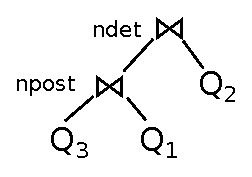
\includegraphics[width=0.5\textwidth]{best_plan}
\caption{Лучший порядок соединения таблиц}
\label{fig:best_plan}
\end{figure}

\clearpage
\section{Физический план}
\begin{figure}[h!]
\centering
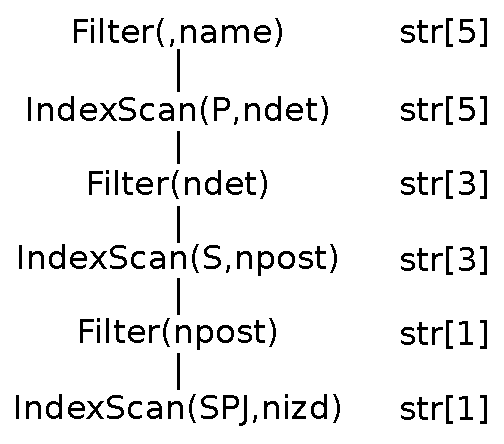
\includegraphics[width=0.9\textwidth]{phys_plan}
\caption{Физический план выполнения запроса}
\label{fig:phys_plan}
\end{figure}

\end{document}